\appendixchapter{\EnergyInteractionModel{}}

\subsection*{Graphical Representation: The \EnergyDiagram{}}

Generic Example involving two physical systems, three energy systems, and with energy added to the system as heat. The \textbf{physical system} consists of \emph{physical thing 1} and \emph{physical thing 2}.

\begin{center}
%	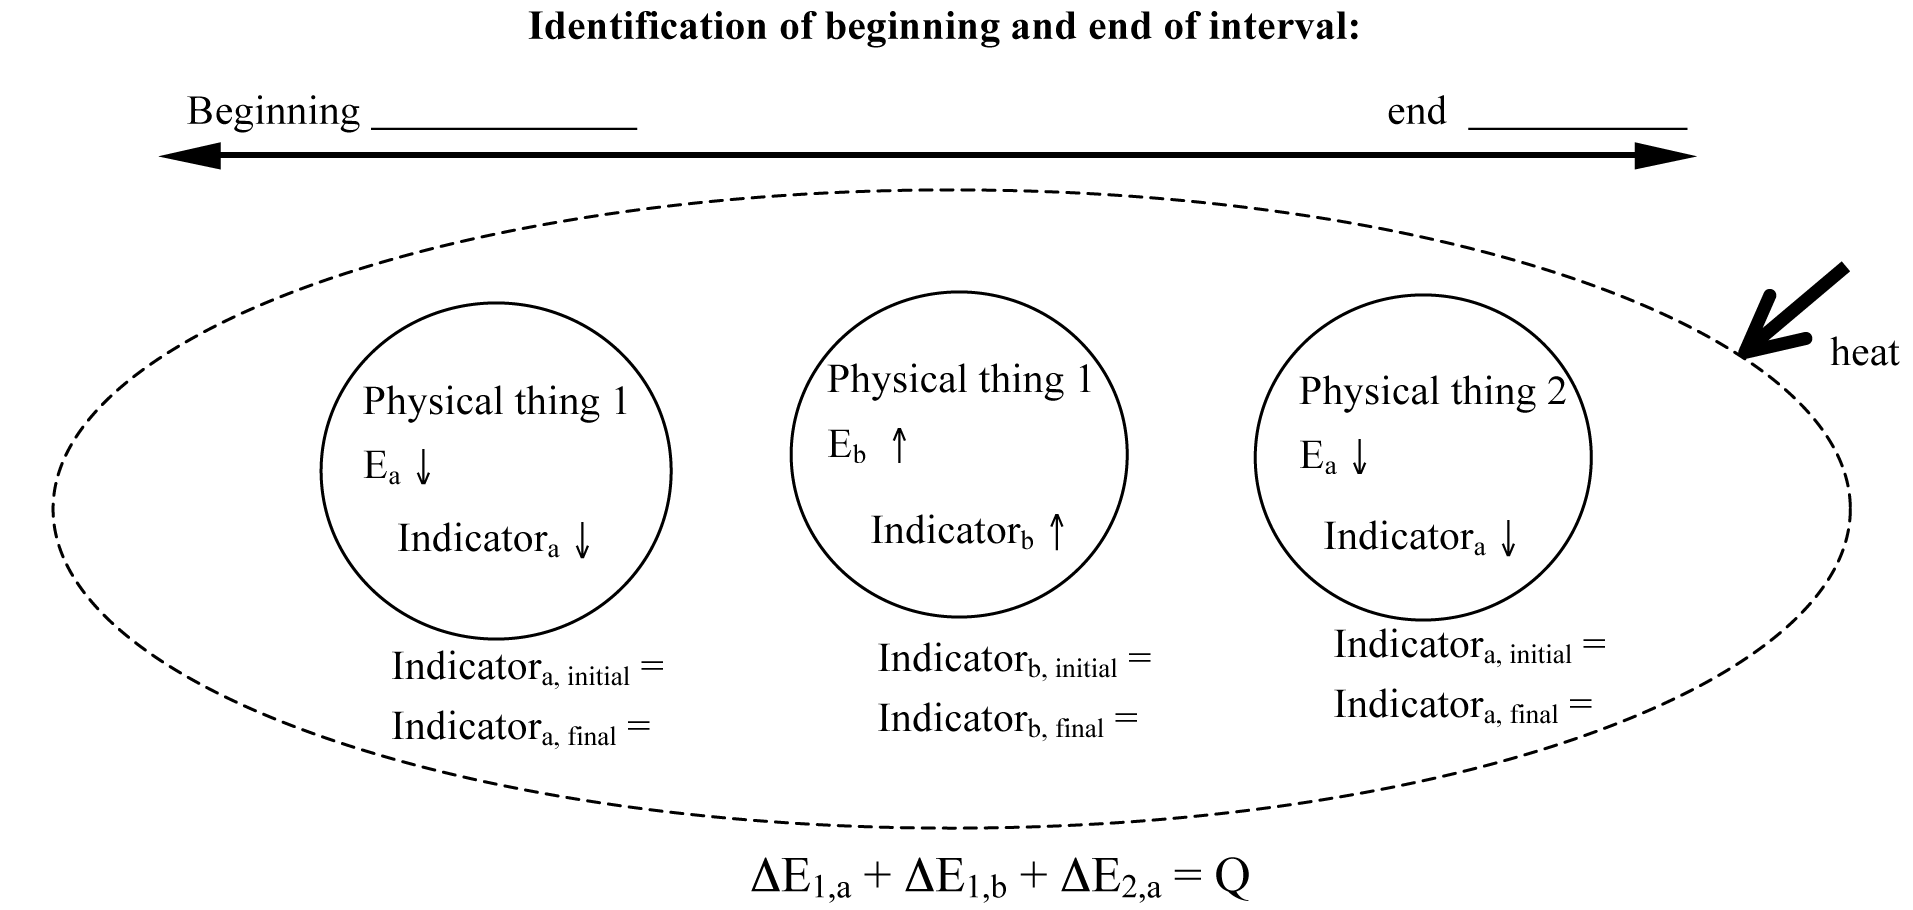
\includegraphics[width=0.8\linewidth]{E-ID}
	
\begin{tikzpicture}
    % draw horizontal line   
    \draw[-{Stealth[scale=1.2]}, line width=1pt] (0,0) -- (10.2,0);

    % draw vertical lines
    \foreach \x in {0.5,9.5}
      \draw[line width=1pt] (\x cm,3pt) -- (\x cm,-3pt);

    % title the diagram
    \draw (5,0) node[above=18pt] {\scriptsize{\textbf{Identification of \emph{beginning} and \emph{end} of interval:}}};

    % draw nodes along the interval timeline
    \draw (0.5,0) node[below=3pt] {\scriptsize{initial conditions}} node[above=3pt] {\emph{beginning}};
    \draw (9.5,0) node[below=3pt] {\scriptsize{final conditions}} node[above=3pt] {\emph{end}};

    % draw the physical system boundary
    \draw [dashed,orange,line width=1pt] (5,-2.75) ellipse (6cm and 2.25cm) node[above=1.5cm] {\textbf{\emph{physical system}}};
    
    % draw energy systems
    \draw (2,-3) node[draw,circle,blue,minimum size=2.25cm,inner sep=0pt,align=center]  {\color{darkgray}\tiny{indicator $a$}\\[.5ex]$\downarrow E_\text{1,a}$\\\color{darkgray}\tiny{$a_i =$}\\[-1.2ex]\color{darkgray}\tiny{$a_f =$}} node[orange,above=1.1cm] {\scriptsize{physical thing 1}};
    \draw (5,-3.25) node[draw,circle,blue,minimum size=2.25cm,inner sep=0pt,align=center]  {\color{darkgray}\tiny{indicator $b$}\\[.5ex]$\uparrow E_\text{1,b}$\\\color{darkgray}\tiny{$b_i =$}\\[-1.2ex]\color{darkgray}\tiny{$a_f =$}} node[orange,above=1.1cm] {\scriptsize{physical thing 1}};
    \draw (8,-3) node[draw,circle,blue,minimum size=2.25cm,inner sep=0pt,align=center]  {\color{darkgray}\tiny{indicator $a$}\\[.5ex]$\downarrow E_\text{2,a}$\\\color{darkgray}\tiny{$a_i =$}\\[-1.2ex]\color{darkgray}\tiny{$a_f =$}} node[orange,above=1.1cm] {\scriptsize{physical thing 2}};    

    % draw heat arrow
    \draw[{Stealth[scale=1.2]}-, line width=1pt, blue] (10,-2.25) -- (11,-1.5)  node[right=0cm] {heat Q};
    
    % write energy conservation equation
    \draw (5,-6) node[] {$\Delta E_\text{1,a} + \Delta E_\text{1,b} + \Delta E_\text{2,a} = Q$};
    \draw (3,-6) node[above=6pt] {\scriptsize{$(-)$}};
    \draw (4.6,-6) node[above=6pt] {\scriptsize{$(+)$}};
    \draw (6.15,-6) node[above=6pt] {\scriptsize{$(-)$}};
    \draw (7.35,-6) node[above=6pt] {\scriptsize{$(+)$}};

\end{tikzpicture}
\end{center}

\subsection*{Algebraic Representations}

\begin{align*}
	\text{Open system:} && \Delta E_\text{total} &= \sum \Delta E_i = \Delta E_1 + \Delta E_2 + \Delta E_3 + \ldots = Q + W \\[5mm]
	\text{Closed system:} && \Delta E_\text{total} &= \sum \Delta E_i = \Delta E_1 + \Delta E_2 + \Delta E_3 + \ldots = 0 \\[5mm]
	\text{Power:} && P &= \frac{\Delta E}{\Delta t}\\[5mm]
%	\text{Work:} && W &= F_\text{parallel} \Delta x = F_{||}\Delta x
\end{align*}

\pagebreak

\renewcommand{\leftcolumn}{0.375\linewidth}
\renewcommand{\rightcolumn}{0.625\linewidth}

\noindent
\parbox[b]{\leftcolumn}{
	\textbf{Constructs}}
\parbox[b]{\rightcolumn}{
	\textbf{Relationships}}

\vspace*{-\parskip}
\noindent
\hrulefill

\vspace*{-\parskip}
\noindent
\parbox[c]{\leftcolumn}{
	\noindent
	Energy
		\\\hspace*{1em}$\bullet$ Conservation of Energy
		\\\hspace*{1em}$\bullet$ Internal Energy ($U$)
		\\\hspace*{1em}$\bullet$ Mechanical Energy
		\\\hspace*{1em}$\bullet$ Energy Transfers ($Q$, $W$)\\

	\noindent
	Physical System
		\\\hspace*{1em}$\bullet$ closed
		\\\hspace*{1em}$\bullet$ open\\
	(with respect to energy transfers)\\

	\noindent
	Energy Transfer
		\\\hspace*{1em}$\bullet$ Heat, $Q$
		\\\hspace*{1em}$\bullet$ Work, $W$\\
	
	\noindent
	Energy System
		\\\hspace*{1em}$\bullet$ Indicators
		\\\hspace*{1em}$\bullet$ Change in Energy ($\Delta E$)\\
			
	\noindent
	Process or Interaction
		\\\hspace*{1em}$\bullet$ Interval
		\\\hspace*{1em}$\bullet$ initial (start) Time of Interval
		\\\hspace*{1em}$\bullet$ final (end) Time of Interval\\
	
	\noindent
	State of a Physical System
		\\\hspace*{1em}$\bullet$ Temperature
		\\\hspace*{1em}$\bullet$ Phase\\
	
	\noindent
	Energy Systems related to Thermal \& Chemical Processes
		\\\hspace*{1em}$\bullet$ $E_\text{thermal}$
		\\\hspace*{1em}$\bullet$ $E_\text{bond}$\\
	
	\noindent
	Energy Systems related to Mechanical Processes
		\\\hspace*{1em}$\bullet$ $PE_\text{gravitational}$
		\\\hspace*{1em}$\bullet$ $PE_\text{elastic}$
		\\\hspace*{1em}$\bullet$ $PE_\text{mass-spring}$
		\\\hspace*{1em}$\bullet$ $KE_\text{translational}$
		\\\hspace*{1em}$\bullet$ $KE_\text{rotational}$
	}
\parbox[c]{\rightcolumn}{
	\begin{enumerate}
		\item The heart of the \EnergyInteractionModel{} is \emph{energy conservation}, one of a few powerful \emph{conservation principles} used throughout science. One way of expressing a conservation principle is that for an isolated physical system, there are certain physical properties that do not change during an interaction or process. A process or interaction is determined by explicitly expressing the beginning and ending times of the interval characterizing the process.
		
		\item The \emph{total energy} of every \emph{physical system} can be expressed as a \emph{sum of the energies} of separately identifiable \emph{energy systems}. This division of the total energy into energy systems can be carried out in multiple ways. The energy associated with a particular energy system can be expressed in terms of \emph{observable} and \emph{measurable properties} of the physical system that we call \emph{indicators}. The \emph{change} in energy of each energy system can be determined from the \emph{observed change in the indicator} that occurs from the beginning to the end of the interval characterizing the interaction or process.
		
		\item Conservation of energy in a \emph{\textbf{closed} physical system} (isolated with respect to energy transfers from other physical systems): The \textbf{total energy} of the physical system must remain \textbf{constant} during the interaction or process. When internal interactions occur, this conservation principle can be expressed in terms of changes within the energy systems of the physical system: The \textbf{changes of the energies of \emph{all energy systems}} associated with the \emph{physical system} in question must \textbf{sum to zero}.
		
		\item Conservation of energy in an \emph{\textbf{open} physical system}: During an interaction or process during which \emph{energy is added or removed} from the physical system as heat or work, the \textbf{changes in energy of {\em all energy systems}} associated with the physical system in question must \textbf{sum to the net energy added (or removed)} as heat and/or work. Equivalently, the \textbf{change in the {\em total energy}} of that physical system must \textbf{equal the net energy added (or removed)} as heat and/or work.
	\end{enumerate}
}
	
\pagebreak

\subsection*{Steps Involved in Using the \EnergyDiagram{}}

\subsubsection*{Prior to writing anything down:}

\begin{benumerate}
	\bitem{Tell a story about what happened!} Be sure you are clear about what the physical phenomenon or process is.
\end{benumerate}

\subsubsection*{Go back and forth through Steps~2-6 until your \EnergyDiagram{} is complete:}

\begin{benumerate}\setcounter{enumi}{1}
	\bitem{What is the boundary of the physical system you are modeling?} What is inside and what is outside?
	\bitem{Is the physical system in your particular model open or closed?} If open, are there any energy transfers (e.g., heat or work)?
	\bitem{What is the extent of the process or interaction?} What determines the beginning and end?
	\bitem{What energy systems do you include in your diagram?} Which indicators are changing?
	\bitem{What are the values of the indicators at the times corresponding to the ends of the time interval you chose in step 4?}
\end{benumerate}

\subsubsection*{Only \emph{after the diagram is complete}, move on to Step~7:}

\begin{benumerate}\setcounter{enumi}{6}
	\bitem{Write down an equation expressing energy conservation for your particular \EnergyDiagram{}, in terms of the $\Delta E$'s and any $Q$ or $W$.} Each term in your conservation of energy equation must correspond to an energy system in your diagram.
\end{benumerate}

\pagebreak

\subsection*{Energy Systems and their Indicators}

\subsubsection*{Energy Systems related to \emph{Thermal \& Chemical Processes}}

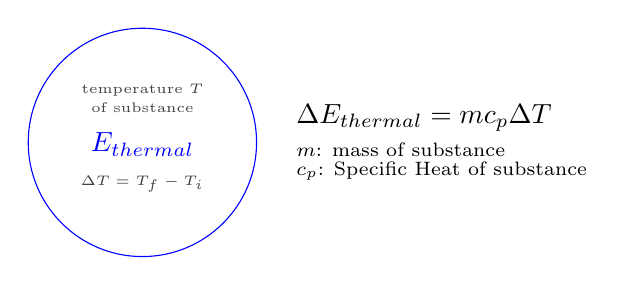
\begin{tikzpicture}
	\node[draw,circle,minimum size=2.9cm,blue,inner sep=0pt, align=center] {\color{darkgray}\tiny{temperature $T$}\\[-1.2ex]\color{darkgray}\tiny{of substance}\\[.5ex]$E_\text{thermal}$\\\color{darkgray}\tiny{$\Delta T = T_f - T_i$}\\[-1.5ex]\hspace{0pt}};
	\node[align=left] at (3.8,0) {$\Delta E_\text{thermal} = m c_p \Delta T$\\\scriptsize{$m$: mass of substance}\\[-1.2ex]\scriptsize{$c_p$: Specific Heat of substance}};
\end{tikzpicture}\\

\noindent
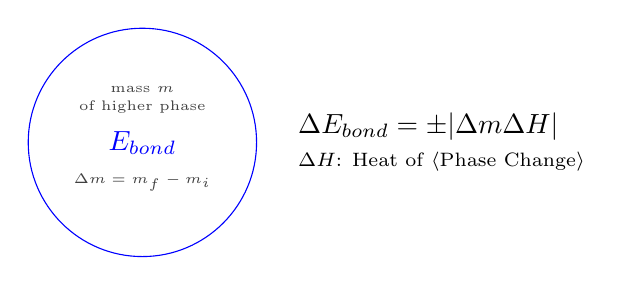
\begin{tikzpicture}
	\node[draw,circle,minimum size=2.9cm,blue,inner sep=0pt, align=center] {\color{darkgray}\tiny{mass $m$}\\[-1.2ex]\color{darkgray}\tiny{of higher phase}\\[.5ex]$E_\text{bond}$\\\color{darkgray}\tiny{$\Delta m = m_f - m_i$}\\[-1.5ex]\hspace{0pt}};
	\node[align=left] at (3.8,0) {$\Delta E_\text{bond} = \pm | \Delta m \Delta H |$\\\scriptsize{$\Delta H$: Heat of $\langle$Phase Change$\rangle$}};
\end{tikzpicture}

\subsubsection*{Energy Systems related to \emph{Mechanical Processes}}

% first column
\begin{minipage}[c]{0.5\textwidth}

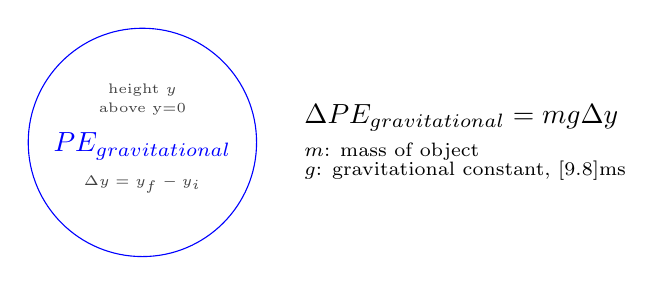
\begin{tikzpicture}
	\node[draw,circle,minimum size=2.9cm,blue,inner sep=0pt, align=center] {\color{darkgray}\tiny{height $y$}\\[-1.2ex]\color{darkgray}\tiny{above y=0}\\[.5ex]$PE_\text{gravitational}$\\\color{darkgray}\tiny{$\Delta y = y_f - y_i$}\\[-1.5ex]\hspace{0pt}};
	\node[align=left] at (4.1,0) {$\Delta PE_\text{gravitational} = m g \Delta y$\\\scriptsize{$m$: mass of object}\\[-1.2ex]\scriptsize{$g$: gravitational constant, \unitfrac[9.8]{m}{s}}};
\end{tikzpicture}\\

\noindent
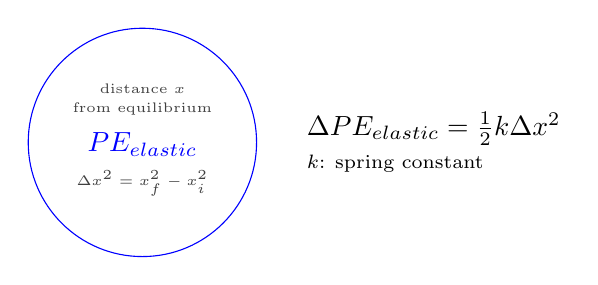
\begin{tikzpicture}
	\node[draw,circle,minimum size=2.9cm,blue,inner sep=0pt,align=center] {\color{darkgray}\tiny{distance $x$}\\[-1.2ex]\color{darkgray}\tiny{from equilibrium}\\[.5ex]$PE_\text{elastic}$\\\color{darkgray}\tiny{$\Delta x^2 = x_f^2 - x_i^2$}\\[-1.5ex]\hspace{0pt}};
	\node[align=left] at (3.7,0) {$\Delta PE_\text{elastic} = \frac{1}{2} k \Delta x^2$\\\scriptsize{$k$: spring constant}};
\end{tikzpicture}\\

\noindent
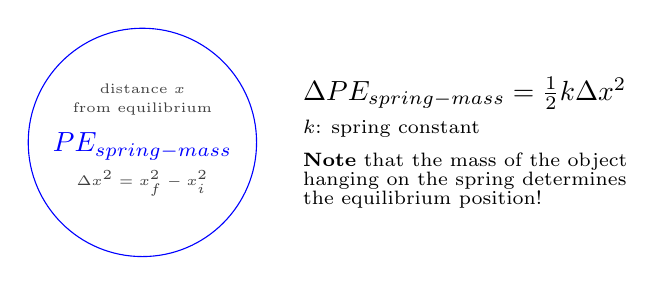
\begin{tikzpicture}
	\node[draw,circle,minimum size=2.9cm,blue,inner sep=0pt,align=center] {\color{darkgray}\tiny{distance $x$}\\[-1.2ex]\color{darkgray}\tiny{from equilibrium}\\[.5ex]$PE_\text{spring-mass}$\\\color{darkgray}\tiny{$\Delta x^2 = x_f^2 - x_i^2$}\\[-1.5ex]\hspace{0pt}};
	\node[align=left] at (4.1,0) {$\Delta PE_\text{spring-mass} = \frac{1}{2} k \Delta x^2$\\\scriptsize{$k$: spring constant}\\\scriptsize{\textbf{Note} that the mass of the object}\\[-1.2ex]\scriptsize{hanging on the spring determines}\\[-1.2ex]\scriptsize{the equilibrium position!}};
\end{tikzpicture}\\
\end{minipage}
%second column
\begin{minipage}[c]{0.5\textwidth}

\noindent
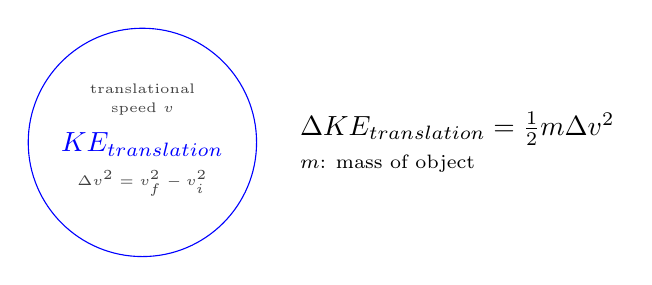
\begin{tikzpicture}
	\node[draw,circle,minimum size=2.9cm,blue,inner sep=0pt,align=center] {\color{darkgray}\tiny{translational}\\[-1.2ex]\color{darkgray}\tiny{speed $v$}\\[.5ex]$KE_\text{translation}$\\\color{darkgray}\tiny{$\Delta v^2 = v_f^2 - v_i^2$}\\[-1.5ex]\hspace{0pt}};
	\node[align=left] at (4,0) {$\Delta KE_\text{translation} = \frac{1}{2} m \Delta v^2$\\\scriptsize{$m$: mass of object}};
\end{tikzpicture}\\

\noindent
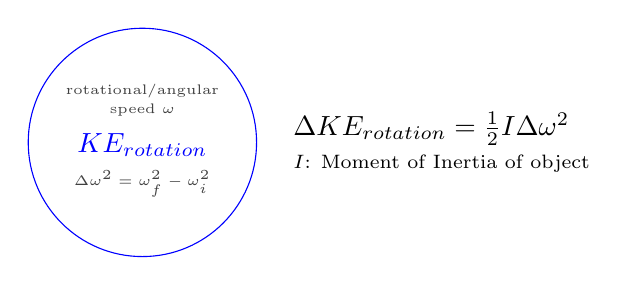
\begin{tikzpicture}
	\node[draw,circle,minimum size=2.9cm,blue,inner sep=0pt, align=center] {\color{darkgray}\tiny{rotational/angular}\\[-1.2ex]\color{darkgray}\tiny{speed $\omega$}\\[.5ex]$KE_\text{rotation}$\\\color{darkgray}\tiny{$\Delta \omega^2 = \omega_f^2 - \omega_i^2$}\\[-1.5ex]\hspace{0pt}};
	\node[align=left] at (3.8,0) {$\Delta KE_\text{rotation} = \frac{1}{2} I \Delta \omega^2$\\\scriptsize{$I$: Moment of Inertia of object}};
\end{tikzpicture}
\end{minipage}

\null